\documentclass[11pt, a4paper]{article}

% --- UNIVERSAL PREAMBLE BLOCK ---
% CHANGED: Switched to 'landscape' and reduced margins to 1cm to fit the wide diagram
\usepackage[a4paper, landscape, top=2cm, bottom=2cm, left=1cm, right=1cm]{geometry}

% Add because main language is not English (Standard safety include)
\usepackage{enumitem}
\setlist[itemize]{label=-}

% --- TIKZ PACKAGES ---
\usepackage{tikz}
\usetikzlibrary{arrows.meta, positioning, calc, shapes.geometric, decorations.markings}

% --- COLOR DEFINITIONS (UofSC Marketing Toolbox) ---
% Primary Colors
\definecolor{UofSCGarnet}{RGB}{115, 0, 10}
\definecolor{UofSCBlack}{RGB}{0, 0, 0}
\definecolor{UofSCWhite}{RGB}{255, 255, 255}

% Neutral Colors
\definecolor{UofSC90Black}{RGB}{54, 54, 54}
\definecolor{UofSC70Black}{RGB}{92, 92, 92}
\definecolor{UofSC50Black}{RGB}{162, 162, 162}
\definecolor{UofSC30Black}{RGB}{199, 199, 199}
\definecolor{UofSC10Black}{RGB}{235, 235, 235}
\definecolor{UofSCWarmGrey}{RGB}{103, 97, 86}
\definecolor{UofSCSandstorm}{RGB}{255, 242, 227}

% Accent Colors
\definecolor{UofSCRose}{RGB}{204, 46, 64}
\definecolor{UofSCAtlantic}{RGB}{70, 106, 159}
\definecolor{UofSCCongaree}{RGB}{31, 65, 77}
\definecolor{UofSCHorseshoe}{RGB}{101, 120, 11}
\definecolor{UofSCGrass}{RGB}{206, 211, 24}
\definecolor{UofSCHoneycomb}{RGB}{164, 145, 55}

% Special Use Colors
\definecolor{UofSCDarkGarnet}{RGB}{87, 0, 8}
\definecolor{UofSCAzalea}{RGB}{132, 66, 71}

\begin{document}

\begin{figure}[htbp]
\centering
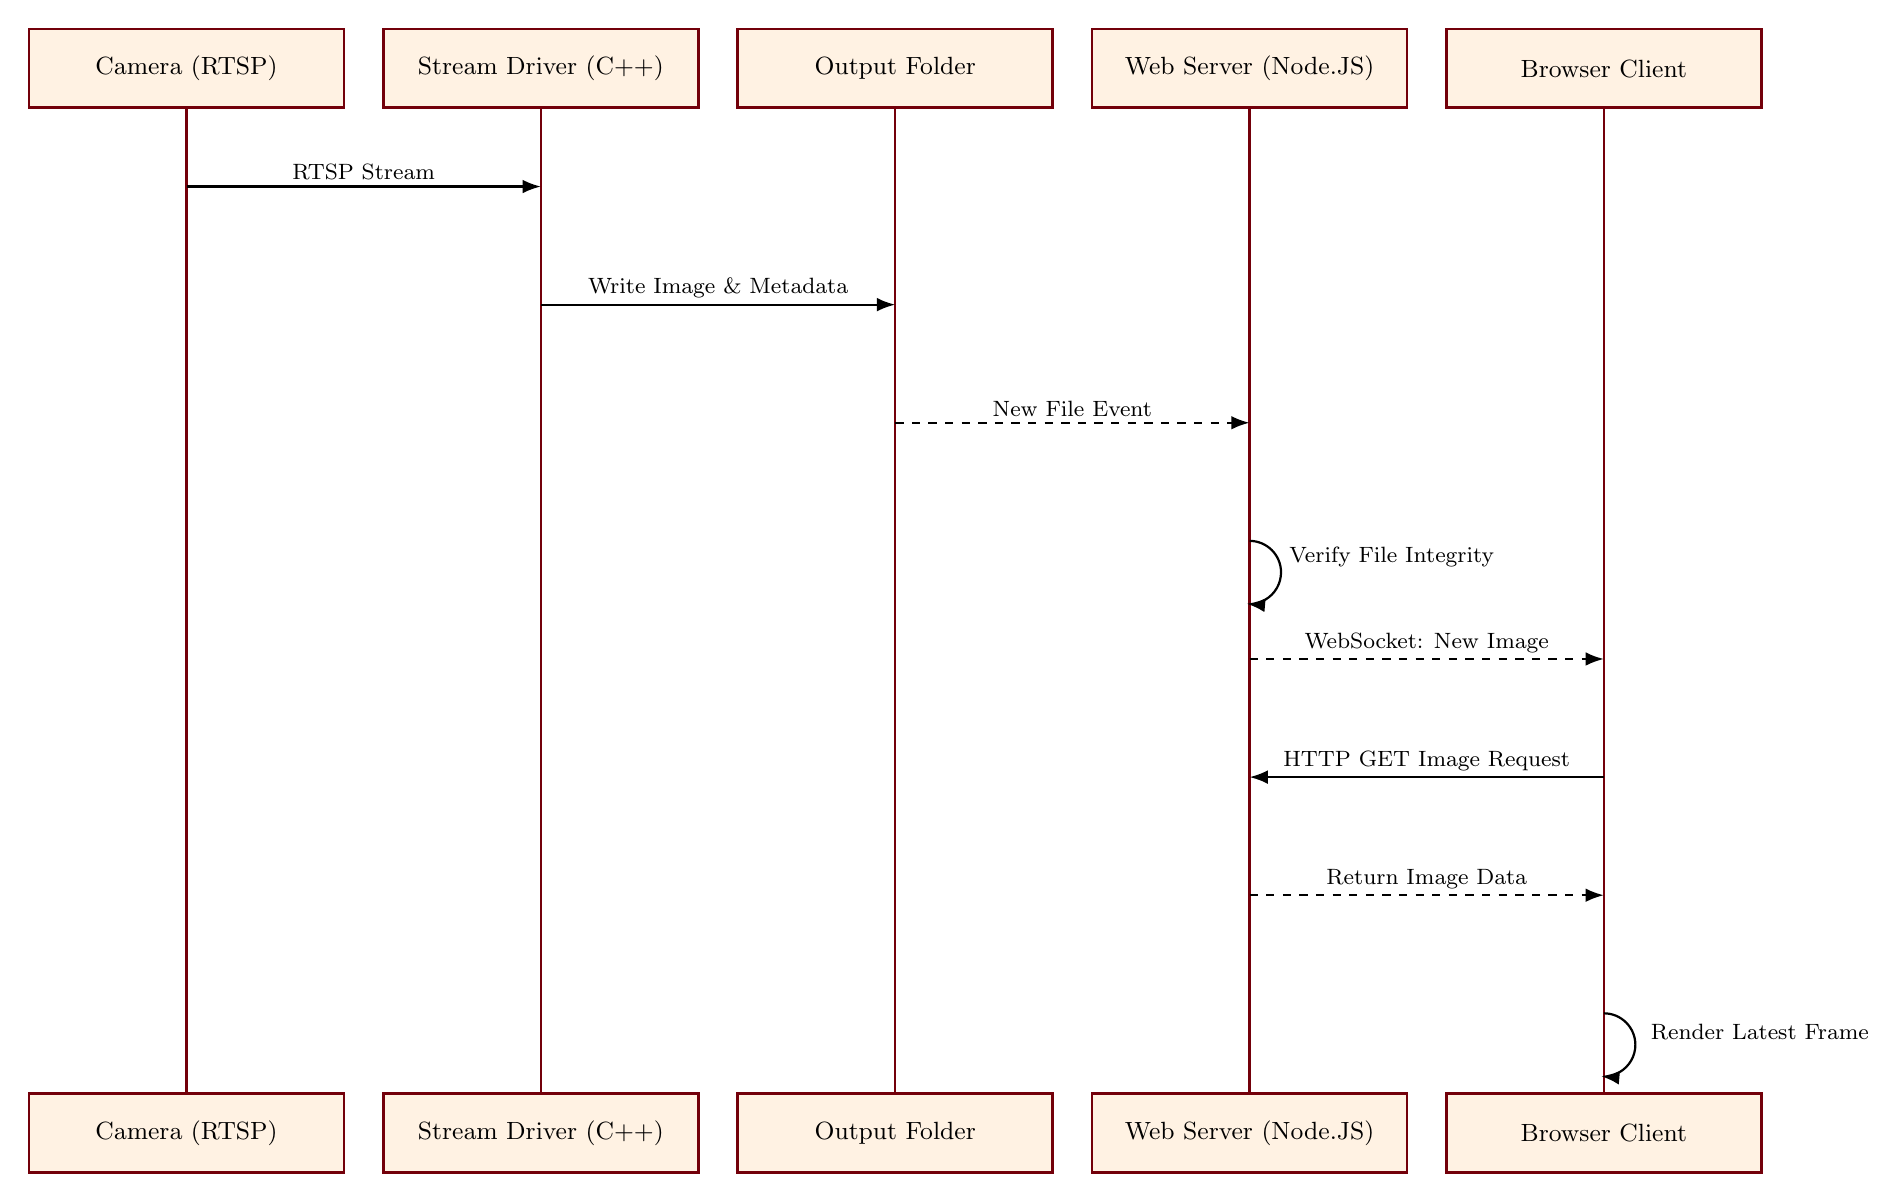
\begin{tikzpicture}[
    node distance=1.5cm and 3cm,
    font=\small,
    participant/.style={
        draw=UofSCGarnet,          % Primary Brand Color for border
        fill=UofSCSandstorm,       % Light neutral for background
        inner sep=8pt, 
        align=center,
        minimum height=1cm,
        minimum width=4cm,
        text=UofSCBlack,           % Standard Black text
        line width=1.0pt           % Slightly thicker border for emphasis
    },
    lifeline/.style={
        draw=UofSCGarnet,          % Vertical lines match the header border
        thick
    },
    message/.style={
        ->, 
        >=Latex, 
        thick, 
        draw=UofSCBlack            % Arrows in high-contrast black
    },
    dashed_message/.style={
        ->, 
        >=Latex, 
        thick, 
        dashed,
        draw=UofSCBlack            % Dashed arrows in high-contrast black
    },
    label_text/.style={
        above, 
        font=\footnotesize,
        align=center,
        inner sep=2pt,
        text=UofSCBlack            % Ensure labels are black
    }
]

    % --- 1. Participants ---
    % Define horizontal positions manually to ensure enough space for long labels
    \node[participant] (camera) at (0,0) {Camera (RTSP)};
    \node[participant] (driver) at (4.5,0) {Stream Driver (C++)};
    \node[participant] (folder) at (9,0) {Output Folder};
    \node[participant] (server) at (13.5,0) {Web Server (Node.JS)};
    \node[participant] (browser) at (18,0) {Browser Client};

    % --- 2. Lifelines (Vertical) ---
    % Define the bottom coordinate based on how long the sequence is
    \coordinate (bottom) at (0,-13);

    \draw[lifeline] (camera.south) -- (camera |- bottom) node[participant, anchor=north] {Camera (RTSP)};
    \draw[lifeline] (driver.south) -- (driver |- bottom) node[participant, anchor=north] {Stream Driver (C++)};
    \draw[lifeline] (folder.south) -- (folder |- bottom) node[participant, anchor=north] {Output Folder};
    \draw[lifeline] (server.south) -- (server |- bottom) node[participant, anchor=north] {Web Server (Node.JS)};
    \draw[lifeline] (browser.south) -- (browser |- bottom) node[participant, anchor=north] {Browser Client};

    % --- 3. Interactions ---

    % Define time steps (y-coordinates)
    \coordinate (t1) at (0,-1.5);
    \coordinate (t2) at (0,-3.0);
    \coordinate (t3) at (0,-4.5);
    \coordinate (t4) at (0,-6.0); % Loop
    \coordinate (t5) at (0,-7.5);
    \coordinate (t6) at (0,-9.0);
    \coordinate (t7) at (0,-10.5);
    \coordinate (t8) at (0,-12.0); % Loop

    % Interaction 1: Camera -> Driver
    \draw[message] (camera |- t1) -- node[label_text] {RTSP Stream} (driver |- t1);

    % Interaction 2: Driver -> Output Folder
    \draw[message] (driver |- t2) -- node[label_text] {Write Image \& Metadata} (folder |- t2);

    % Interaction 3: Output Folder -> Server (Dashed)
    \draw[dashed_message] (folder |- t3) -- node[label_text] {New File Event} (server |- t3);

    % Interaction 4: Server Self-Loop
    % UPDATED: Using 'arc' for a perfect semi-circle on the right
    \draw[message] (server |- t4) 
        arc[start angle=90, end angle=-95, radius=0.4] 
        node[midway, right=40pt, label_text, align=left] {Verify File Integrity};

    % Interaction 5: Server -> Browser (Dashed)
    % Note: t5 needs to be below the loop. t4 loop ends at roughly -6.6
    \draw[dashed_message] (server |- t5) -- node[label_text] {WebSocket: New Image} (browser |- t5);

    % Interaction 6: Browser -> Server
    \draw[message] (browser |- t6) -- node[label_text] {HTTP GET Image Request} (server |- t6);

    % Interaction 7: Server -> Browser (Dashed)
    \draw[dashed_message] (server |- t7) -- node[label_text] {Return Image Data} (browser |- t7);

    % Interaction 8: Browser Self-Loop
    % UPDATED: Using 'arc' for a perfect semi-circle on the left
    \draw[message] (browser |- t8) 
        arc[start angle=90, end angle=-95, radius=0.4] 
        node[midway, right=45pt, label_text, align=right] {Render Latest Frame};

\end{tikzpicture}

\end{figure}

\end{document}